\documentclass[11pt]{article}
\usepackage[margin=0.75in]{geometry}
\usepackage{amsmath,amssymb,amsthm,booktabs,tikz}
\usepackage[hidelinks]{hyperref}
\newtheorem{theorem}{Theorem}
\newcommand{\Pp}{P_G}
\title{Counterexamples to the convexity strengthening\\of the Merino--Welsh conjecture}
\author{Luis Gonzalez}
\date{26 November 2026}
\begin{document}
\maketitle
\begin{abstract}
Conde and Merino conjectured that the restriction of the Tutte polynomial of a simple, loopless, 2-connected graph to the segment joining $(2,0)$ and $(0,2)$ is convex. We give a graph on 19 vertices and 30 edges for which the second derivative of the restriction at zero is $-6556$. An exact rational midpoint inequality certifies failure of convexity. We also construct a simple planar graph of maximum degree four whose restriction fails even quasiconvexity, and a family in which the ratio of an interior value to the larger of two surrounding values grows exponentially. The finite 19-vertex witness has a Lean 4 certificate. Historical priority remains unresolved.
\end{abstract}
\section{Introduction}
For a finite graph $G=(V,E)$, let $k(A)$ denote the number of components of $(V,A)$, including isolated vertices. We use the convention
\[
T_G(x,y)=\sum_{A\subseteq E}(x-1)^{k(A)-k(E)}(y-1)^{|A|-|V|+k(A)}.
\]
The endpoint inequality originates with Merino and Welsh \cite{MW}. Conjecture 2.4 of Conde and Merino \cite{CM} asserts convexity of $P_G(x)=T_G(x,2-x)$ on $[0,2]$ for every simple, loopless, 2-connected graph. This would imply the additive endpoint inequality $T_G(2,0)+T_G(0,2)\ge 2T_G(1,1)$ for this graph class and hence the corresponding Merino--Welsh inequality. The counterexamples below concern convexity, not the original endpoint conjecture or its additive or multiplicative variants. Convexity is known for coloopless paving matroids \cite{CL} and minimally 2-edge-connected graphs \cite{Ok}; our examples lie outside these classes.

\begin{theorem}\label{thm:small}
Let $G$ consist of a $K_5$ with a chain of five squares joining two distinct vertices $s,t$ of the clique, with opposite corners as terminals in each square. Keep all clique edges. Then $G$ is simple and 2-connected, and
\[
P_G(x)=280024+5612x-3278x^2+O(x^3).
\]
In particular $P_G''(0)=-6556$, and $P_G$ is not convex on $[0,2]$.
\end{theorem}
\begin{center}
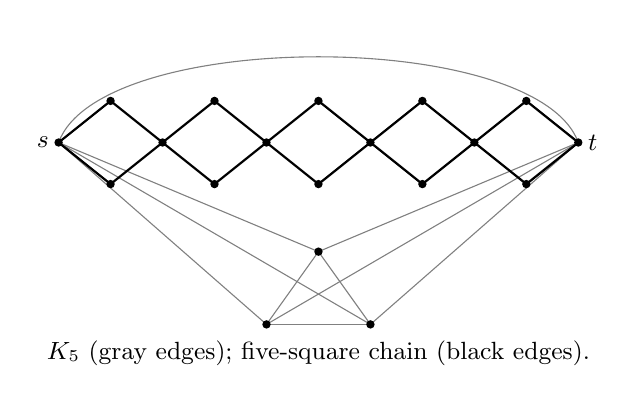
\begin{tikzpicture}[scale=.66,every node/.style={font=\small}]
\coordinate (s) at (0,0); \coordinate (t) at (10,0);
\coordinate (a) at (5,-2.1); \coordinate (b) at (4,-3.5); \coordinate (c) at (6,-3.5);
\foreach \i/\j in {s/a,s/b,s/c,t/a,t/b,t/c,a/b,a/c,b/c}{\draw[gray] (\i)--(\j);}
\draw[gray] (s) to[out=70,in=110,looseness=0.6] (t);
\foreach \i in {0,...,4}{\pgfmathtruncatemacro{\j}{\i+1}\draw[thick] (2*\i,0)--(2*\i+1,.8)--(2*\j,0)--(2*\i+1,-.8)--cycle;\fill (2*\i+1,.8) circle(2.3pt);\fill (2*\i+1,-.8) circle(2.3pt);}
\foreach \i in {0,...,5}{\fill (2*\i,0) circle(2.3pt);}
\foreach \i in {a,b,c}{\fill (\i) circle(2.3pt);}
\node[left] at (s) {$s$};\node[right] at(t){$t$};\node at (5,-4.05) {$K_5$ (gray edges); five-square chain (black edges).};
\end{tikzpicture}
\end{center}
\section{A finite convexity counterexample}
\begin{proof}[Proof of Theorem \ref{thm:small}]
The chain adds four junctions and ten internal vertices, so $|V|=19$ and $|E|=30$. The graph is obtained from the clique by adding a ten-edge ear between $s,t$ and then adding a two-edge ear parallel to each successive two-edge section. An ear has distinct existing endpoints and fresh internal vertices. Adding such an ear preserves simplicity and 2-vertex-connectivity: after deleting one vertex, each surviving part of the ear meets the connected remainder. 

For any connected graph $J$ with distinct vertices $v,w$, write $J/vw$ for their identification, retaining loops and parallel edges. Adding a two-edge path from $v$ to $w$ gives $(1+x)P_J+P_{J/vw}$ by deletion--contraction. Apply the same rule to a second two-edge path. After identifying $v,w$, the first path becomes a two-edge cycle attached at one vertex, whose Tutte evaluation is $x+(2-x)=2$. Thus adding a square between opposite corners gives
\begin{equation}\label{eq:square}
(1+x)^2P_J+(3+x)P_{J/vw}.
\end{equation}
Here the Tutte polynomial is multiplicative under a one-vertex union, directly from the subset formula.

Let $A_i$ denote the polynomial of the clique with an open chain of $i$ squares attached at $s$, and $B_i$ the polynomial after identifying its free end with $t$. For $i=0$ the free end is $s$. A one-vertex square attachment multiplies by $T_{C_4}(x,2-x)=2+x^2+x^3$. By \eqref{eq:square},
\begin{equation}\label{eq:rec}
A_{i+1}=(2+x^2+x^3)A_i,\qquad
B_{i+1}=(1+x)^2A_i+(3+x)B_i,\qquad P_G=B_5.
\end{equation}
The initial polynomials are $A_0=P_{K_5}$ and $B_0=P_{K_5/st}$. Their coefficients in increasing degree are
\begin{align*}
A_0:&\quad 544,-932,796,-374,106,-16,1,\\
B_0:&\quad 680,-1680,1898,-1240,499,-123,17,-1.
\end{align*}
These follow by summing over the $2^{10}$ subsets of the labelled clique edges: each summand is $(-1)^{k-1}(1-x)^{k-1+j}$, with $j=|A|-n+k$. For $A_0$ use $n=5$; for $B_0$ identify $s,t$ before counting components and use $n=4$. The first three coefficients in the recurrence are
\begin{center}
\begin{tabular}{r rr}
\toprule
$i$ & $A_i$ & $B_i$\\\midrule
0 & $544,-932,796$ & $680,-1680,1898$\\
1 & $1088,-1864,2136$ & $2584,-4204,3490$\\
2 & $2176,-3728,5360$ & $8840,-9716,5762$\\
3 & $4352,-7456,12896$ & $28696,-19684,7650$\\
4 & $8704,-14912,30144$ & $90440,-29108,5602$\\
5 & $17408,-29824,68992$ & $280024,5612,-3278$\\\bottomrule
\end{tabular}
\end{center}
Consequently $P_G''(0)=-6556$; continuity gives negative curvature at interior points. Alternatively, evaluating \eqref{eq:rec} at $h=1/256$ gives the exact midpoint certificate
\begin{equation}\label{eq:gap}
2P_G(h)-P_G(0)-P_G(2h)
=\frac{26123280769243048353292998299952433382036731393}{2^{159}}>\frac1{32}.
\end{equation}
Convexity requires the left-hand side to be nonpositive.
\end{proof}
\section{Planar counterexamples to quasiconvexity}
\begin{theorem}\label{thm:planar}
There exists a simple planar 2-connected graph $G$ of maximum degree four, on 102 vertices and 151 edges, such that
\[
1000P_G(1/8)>1002P_G(0),\qquad 1000P_G(1/8)>1004P_G(1/4).
\]
In particular the restriction is not quasiconvex. Moreover, for the rings described below with $k=4r$ ordinary and $j=3r$ diagonal cells, the ratio $P_G(1/5)/\max\{P_G(1/10),P_G(3/10)\}$ grows exponentially as $r\to\infty$.
\end{theorem}
Make a ring of $k+j$ squares whose opposite terminals are shared with the preceding and following cells. Add a diagonal between the two unshared corners in $j$ of the cells. Take $k=19$, $j=15$, in consecutive blocks. Each cell has two unshared vertices and contributes one junction, so there are $3(k+j)$ vertices and $4k+5j$ edges. Planarity follows by drawing the two paths and optional diagonal in a small region around each side of a polygon. A cycle using one two-edge path per cell, followed by ear additions of the other paths, proves 2-connectivity; adding diagonals preserves it. Maximum degree is four.
\begin{center}
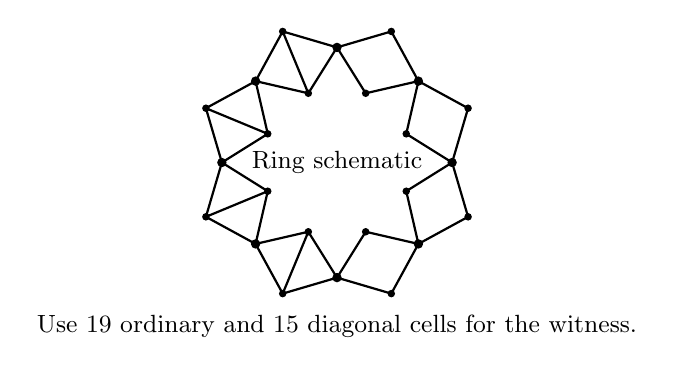
\begin{tikzpicture}[scale=.68,every node/.style={font=\small}]
\foreach \i in {0,...,7}{\coordinate (v\i) at ({90-45*\i}:2.15);}
\foreach \i in {0,...,7}{\pgfmathtruncatemacro{\j}{mod(\i+1,8)}\coordinate (a\i) at ({67.5-45*\i}:2.65);\coordinate (b\i) at ({67.5-45*\i}:1.40);\draw[thick] (v\i)--(a\i)--(v\j)--(b\i)--cycle;\ifnum\i>3\draw[thick] (a\i)--(b\i);\fi\fill (a\i) circle(2pt);\fill (b\i) circle(2pt);\fill (v\i) circle(2.5pt);}
\node at (0,0) {Ring schematic};\node at (0,-3.05) {Use 19 ordinary and 15 diagonal cells for the witness.};
\end{tikzpicture}
\end{center}
Put $u=1-x>0$. For a two-terminal cell, write $C$ for the sum of Tutte subset terms whose terminals are connected and $-uD$ for the sum when they are separated. Its ordinary evaluation is $V=C-uD$. Each subset contributes $(-u)^{k(A)-1}u^{|A|-|V(G)|+k(A)}$. The two cell types give
\begin{center}
\begin{tabular}{lcc}\toprule
Cell & $C$ & $V$\\\midrule
Square & $3+x$ & $2+x^2+x^3$\\
Square with diagonal & $12-5x+x^2$ & $6+x^2+x^3$\\\bottomrule
\end{tabular}
\end{center}
For the square, connected-terminal subsets comprise two two-edge paths, four trees and the full square, yielding $-2u+4+u$. The ordinary evaluation is that of a cycle. Deleting the diagonal leaves the square, while contracting it gives two pairs of parallel edges in series. The connected-terminal contribution of the contracted graph is $(2+u)^2$ and its ordinary evaluation is $4$, giving the second row.

If all cells connect their terminals, closing the ring adds a cycle and contributes $u\prod C_i$. If $h\ge1$ cells separate their terminals, the ring of junctions has $h$ components and no cycle, contributing $(-u)^{h-1}$ in addition to the local factors $D_i,C_i$. Summation over the nonempty choices gives $(\prod C_i-\prod V_i)/u$. Therefore
\begin{equation}\label{eq:ring}
P_G(x)=\frac{(1+u^2)(3+x)^k(12-5x+x^2)^j
 -(2+x^2+x^3)^k(6+x^2+x^3)^j}{u}.
\end{equation}
For an integer-only check write $x=p/q$ and define
\[
a=3q+p,\quad b=12q^2-5pq+p^2,\quad e=2q^3+p^2q+p^3,\quad f=6q^3+p^2q+p^3.
\]
Then the right side of \eqref{eq:ring} is
\[
\frac{(q^2+(q-p)^2)a^k b^j q^{2k+j-2}-e^k f^j}{(q-p)q^{3(k+j)-1}}.
\]
Substituting $(p,q)=(0,8),(1,8),(2,8)$, $k=19$, $j=15$, and cross-multiplying yields the strict inequalities of Theorem \ref{thm:planar}.

For the family use $k=4r$, $j=3r$. The connected product per unit, in the variable $u$, is $F(u)=(4-u)^4(8+3u+u^2)^3$. Its derivative has the sign of $4+3u-10u^2$ on $(0,1)$, so $F$ has a strict maximum at $u=4/5$. Both ordinary cell evaluations are positive and smaller than the connected evaluations on $(0,1)$: the differences are $u(2-u)^2$ and $u(8-3u+u^2)$ respectively. Formula \eqref{eq:ring} gives $P_G(1-u)^{1/r}\to F(u)$. Comparing $u=7/10,4/5,9/10$ proves the exponentially growing interior-to-surrounding-value ratio and completes the theorem.
\section{Verification, scope and priority}
The \href{https://github.com/Luisproofs/conde-merino-convexity-disproof}{public repository} contains the proofs and reproducible computations. Run \texttt{finite/verify.py} with Python 3 for the finite witnesses. For an independent rank--nullity check, run \texttt{subset\_check.py} in the \texttt{lean/tools/} directory. The latter accounts for all $2^{30}$ edge subsets by grouping them. In \texttt{lean/}, with the pinned Lean 4.36.0 toolchain, run \texttt{lake build} and \texttt{lake env lean Audit.lean}; the Lean README supplies the fresh-kernel replay command. The supplied audit records successful kernel replay and only the standard axioms \texttt{propext}, \texttt{Classical.choice}, and \texttt{Quot.sound}. The updated Lean source proves the identity between deletion--contraction and the rank-subset definition for finite undirected multigraphs (\href{https://github.com/Luisproofs/conde-merino-convexity-disproof/blob/main/lean/CondeMerino/RankSubset.lean}{\texttt{tutte\_eq\_classicalTutte}}), and the finite certificate \eqref{eq:gap} for that definition. The supplied build and replay logs include this theorem. The planar result and infinite family have conventional proofs, not Lean formalizations. A separate large-girth construction is given in the repository (\texttt{convexity-proof.md}).

The 2019 conference paper by Hiraishi et al. \cite{H} has a directly relevant title, but its full text was not available in our investigation; the accessible project report does not settle whether its graph hypotheses and line segment agree with Conjecture 2.4. Recent work \cite{V} discusses convexity in connection with Merino--Welsh. No claim of historical priority or minimality is made. The work is unrefereed.

\paragraph{AI disclosure.} Research directed by Luis Gonzalez, with Astra 6.2 through OpenAI Codex used for discovery, proof development, computation and formalization. Additional AI-assisted review and manuscript preparation were used. Contact: \href{mailto:nftprogrammer@gmail.com}{\nolinkurl{nftprogrammer@gmail.com}}; \url{https://x.com/100xluis}.
\begin{thebibliography}{9}
\bibitem{CM} R. Conde and C. Merino, Comparing the Number of Acyclic and Totally Cyclic Orientations with that of Spanning Trees of a Graph, \emph{International Journal of Mathematical Combinatorics} 2 (2009), 79--89. \url{https://www.matem.unam.mx/~merino/online_papers/conjecture_5.pdf}.
\bibitem{H} H. Hiraishi, H. Imai, S. Moriyama, S. Okamura and S. Shiroshita, Smallest Counterexamples for Convexity and Log-concavity of the Tutte Polynomial, proceedings of the 11th Hungarian--Japanese Symposium (2019). Full text not consulted; see the \href{https://www.opt.mist.i.u-tokyo.ac.jp/hj2019/wp-content/uploads/sites/3/2019/04/program19.pdf}{conference program} and \href{https://kaken.nii.ac.jp/ja/file/KAKENHI-PROJECT-16K12392/16K12392seika.pdf}{project report}.
\bibitem{V} B. V\'ali, The Merino--Welsh conjecture for sparse and dense graphs, arXiv:2611.15008 (2026), \url{https://arxiv.org/abs/2611.15008}.
\bibitem{MW} C. Merino and D. J. A. Welsh, Forests, colourings and acyclic orientations of the square lattice, \emph{Annals of Combinatorics} 3 (1999), 417--429.
\bibitem{CL} L. E. Ch\'avez-Lomel\'i, C. Merino, S. D. Noble and M. Ram\'irez-Ib\'a\~nez, Some inequalities for the Tutte polynomial, \emph{European Journal of Combinatorics} 32 (2011), 422--433. \url{https://doi.org/10.1016/j.ejc.2010.11.005}.
\bibitem{Ok} S. Ok, \emph{Aspects of the Tutte polynomial}, PhD thesis, Technical University of Denmark, 2016, Chapter 6. \url{https://orbit.dtu.dk/en/publications/aspects-of-the-tutte-polynomial/}.
\end{thebibliography}
\end{document}
